\documentclass[11pt]{article}
\usepackage[a4paper,margin=0.82in]{geometry}
\usepackage{fontspec}
\usepackage{xeCJK}
\usepackage{graphicx}
\usepackage{booktabs}
\usepackage{caption}
\usepackage{array}

\setmainfont{Times New Roman}
\setsansfont{Arial}
\setCJKmainfont{Songti SC}
\setCJKsansfont{STHeiti}
\setlength{\parskip}{0.62em}
\setlength{\parindent}{0pt}

\title{Traditional 与 Learning-based 事件表示更新对比报告}
\author{}
\date{2026-05-08}

\begin{document}
\sloppy
\maketitle

\paragraph{实验范围与读数原则。} 本报告更新了 N-MNIST learning-based 结果，并保留 N-Caltech101 与 MVSEC 的既有对比。为了避免混淆，N-MNIST 被分成两类结果：第一类是完整官方测试集或仓库记录的 full-result，对应传统方法和仓库已有 EvRepSL；第二类是本次新跑的 7 个 learning-based sanity-scale 结果，设置为 CPU、10 epoch、train/test limit 2048/512、batch size 32、learning rate 0.0001。这组 sanity 结果可以证明代码路径、表示构建和分类器训练是通的，但不应被当作完整 official-split benchmark 结论。

\begin{figure}[t]
  \centering
  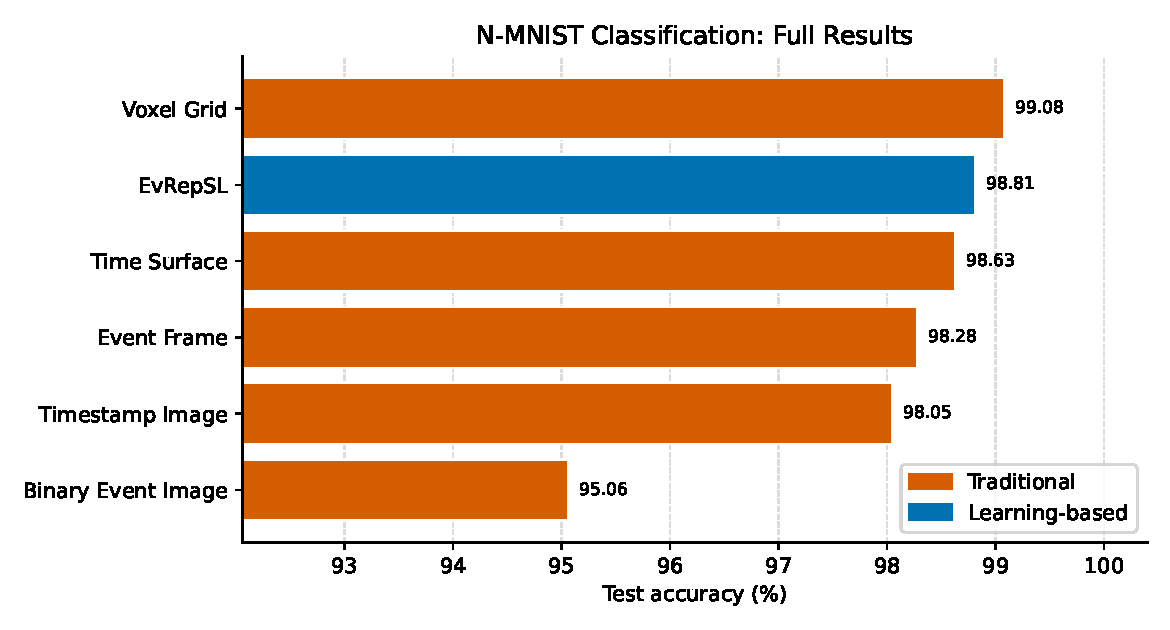
\includegraphics[width=0.86\linewidth]{nmnist_full_accuracy_updated.pdf}
  \caption{N-MNIST 完整结果准确率对比。橙色为 traditional baseline，蓝色为仓库已有 learning-based full result。}
  \label{fig:nmnist-full}
\end{figure}

\paragraph{N-MNIST Full Result Saturation.} 在完整 N-MNIST 结果中，最佳 traditional 方法是 Voxel Grid，准确率为 99.08\%；仓库已有 learning-based EvRepSL 为 98.81\%。二者差距只有 0.27 个百分点，Time Surface、Event Frame 和 Timestamp Image 也均处在 98\% 以上。因此，N-MNIST 更适合作为接口和训练流程验证任务，而不是强区分表示能力的核心任务。Binary Event Image 为 95.06\%，是完整 N-MNIST 中唯一明显掉队的方法，说明只保留二值触发信息会损失一部分时序和强度线索。

\begin{figure}[t]
  \centering
  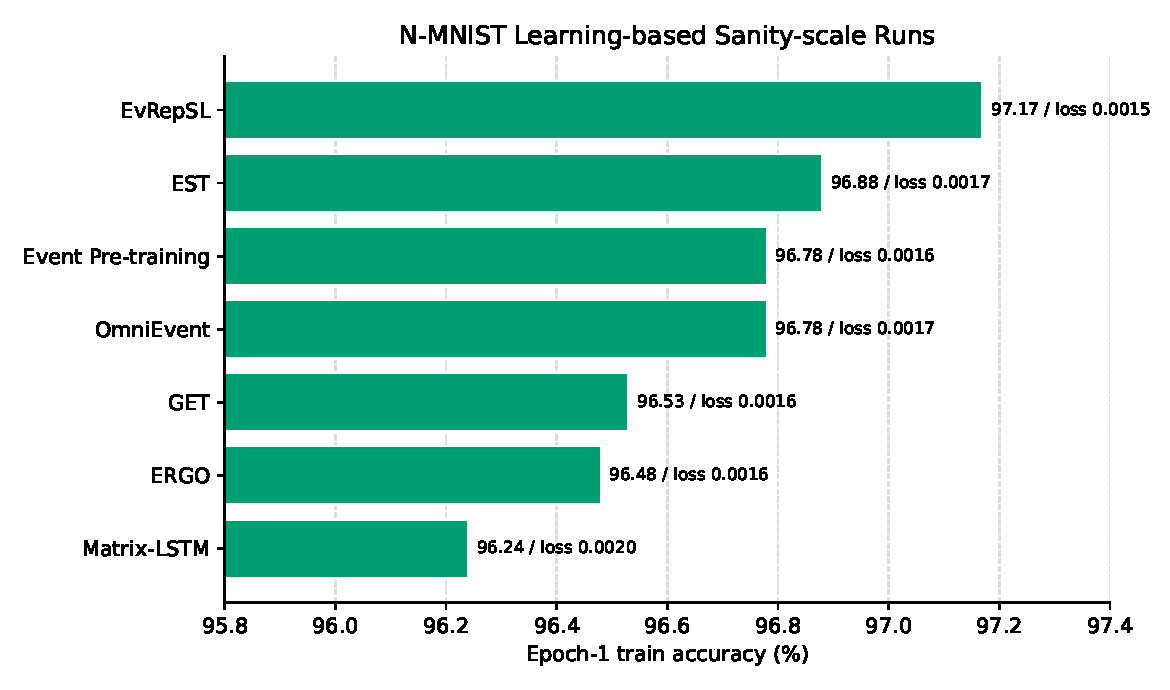
\includegraphics[width=0.86\linewidth]{nmnist_learning_sanity_epoch1.pdf}
  \caption{新跑 N-MNIST learning-based sanity-scale 结果。所有方法在 2048/512 小规模划分上达到 100\% test accuracy，因此图中展示 epoch-1 train accuracy 和最终 train loss，用于观察收敛速度而非最终排名。}
  \label{fig:nmnist-sanity}
\end{figure}

\paragraph{N-MNIST Sanity Runs Are Not Ranking Evidence.} 本次新增的 7 个 learning-based 本地结果在 2048/512 小规模 N-MNIST 设置上全部达到 100.00\% test accuracy，这说明这些方法的本地 adapter、表示张量和 ResNet18 classifier 路径均能正常工作。但由于测试样本只有 512 个，且 N-MNIST 本身接近饱和，这组结果不能用于声称某个 learning-based 方法显著优于另一个方法。若只看训练早期，EvRepSL 的 epoch-1 train accuracy 最高，为 97.17\%；最终 train loss 最低的也是 EvRepSL，为 0.0015。这更像是收敛速度差异，而不是泛化能力差异。

\begin{figure}[t]
  \centering
  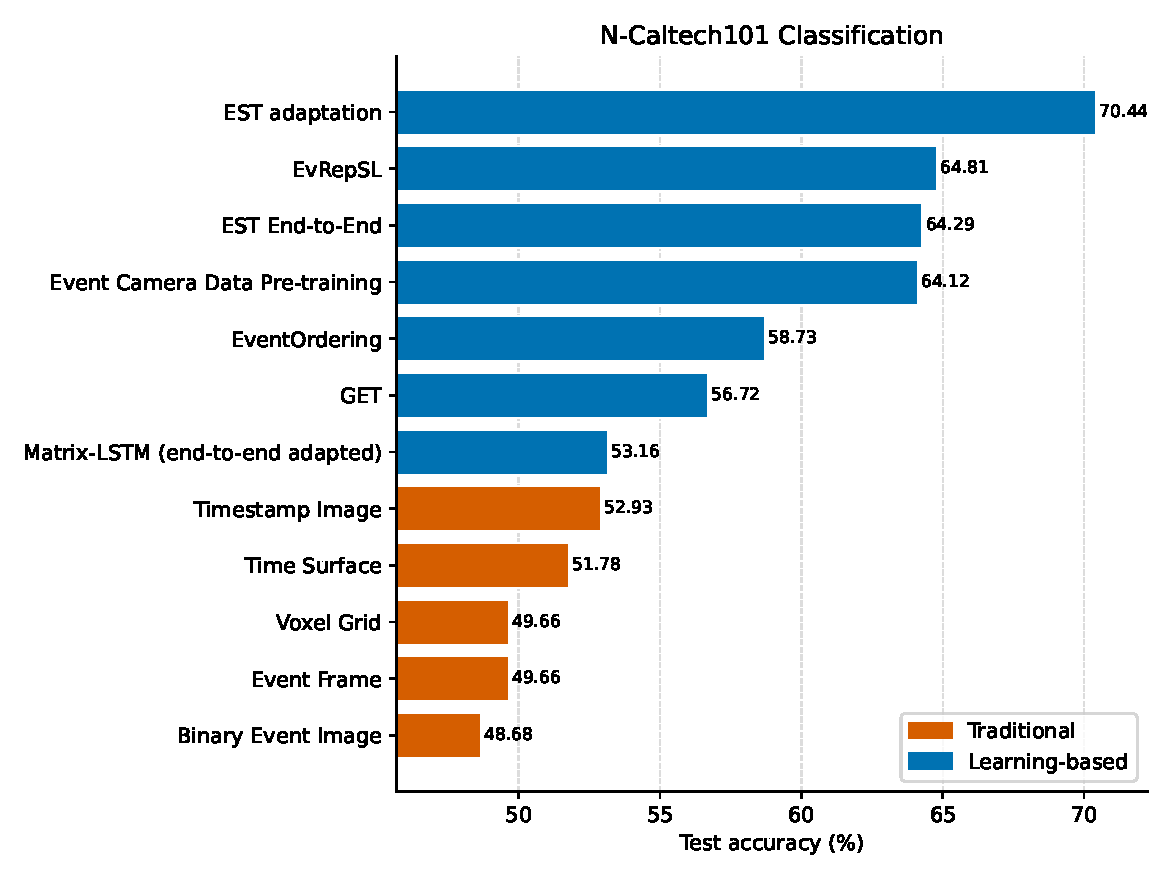
\includegraphics[width=0.92\linewidth]{ncaltech101_accuracy_updated.pdf}
  \caption{N-Caltech101 分类准确率对比。蓝色为 learning-based 方法，橙色为 traditional baseline。}
  \label{fig:ncaltech}
\end{figure}

\paragraph{N-Caltech101 Separates Representation Capacity.} 与 N-MNIST 不同，N-Caltech101 对表示能力的区分更明显。当前最佳 learning-based 方法是 EST adaptation，准确率为 70.44\%；最佳 traditional 方法是 Timestamp Image，准确率为 52.93\%。二者相差 17.51 个百分点。这个差距说明，在类别更多、形状更复杂的事件分类任务上，学习型表示或端到端学习 pipeline 更容易组织跨时间的判别信息；traditional baseline 仍然重要，但更适合作为非学习表示下界。

\begin{figure}[t]
  \centering
  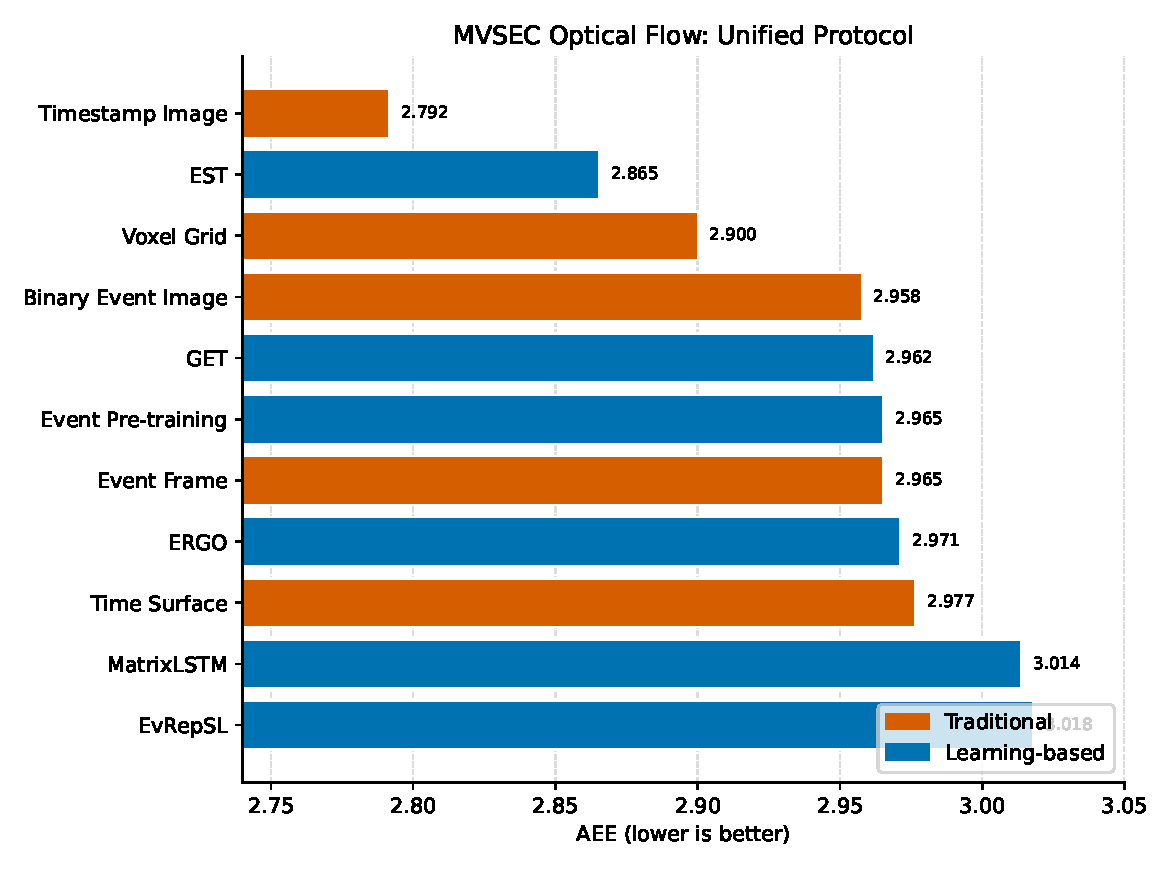
\includegraphics[width=0.88\linewidth]{mvsec_aee_updated.pdf}
  \caption{MVSEC optical flow 统一协议下的 AEE 对比。AEE 越低越好，横轴采用局部放大以展示 2.79--3.02 区间内的差异。}
  \label{fig:mvsec}
\end{figure}

\paragraph{MVSEC Shows A Different Pattern.} MVSEC optical flow 使用 outdoor\_day1/2 训练、indoor\_flying1/2/3 测试，并共享 EVFlowNet-like decoder，因此比分类任务更接近统一协议比较。在这个设置下，最佳方法是 Timestamp Image，AEE 为 2.7916，outlier rate 为 36.61\%；最佳 learning-based 方法是 EST，AEE 为 2.8654。这说明 timestamp-preserving traditional representation 在光流估计中具有很强竞争力。需要谨慎表述的是，这并不等价于 traditional 方法在原论文完整 setting 中全面超过 learning-based 方法，而是在本仓库统一 decoder 和统一 early-stopping protocol 下取得了更低 AEE。

\paragraph{汇报建议。} 晚上汇报可以采用三句话主线。第一，N-MNIST 基本接近饱和，完整结果中 Voxel Grid 与 EvRepSL 仅差 0.27 个百分点，新跑的 7 个 learning-based sanity 结果全部达到 100\%，因此它主要证明 pipeline 可运行。第二，N-Caltech101 才更能拉开差距，EST adaptation 比最佳 traditional Timestamp Image 高 17.51 个百分点，说明复杂分类任务上 learning-based 表示优势更明显。第三，MVSEC 呈现不同结论：统一协议下 Timestamp Image 的 AEE 低于当前 learning-based 最优 EST，说明传统事件表示并不是弱 baseline，尤其保留时间戳结构的表示值得在 survey 中重点讨论。

\end{document}
